
% Template de matriz
% \[
% \begin{bmatrix} % Matriz con linea rectangular
% \begin{pmatrix} % Matriz con linea redonda
%     x_{11} & x_{12} & x_{13} & \dots  & x_{1n} \\
%     x_{21} & x_{22} & x_{23} & \dots  & x_{2n} \\
%     \vdots & \vdots & \vdots & \ddots & \vdots \\
%     x_{d1} & x_{d2} & x_{d3} & \dots  & x_{dn}
% \end{pmatrix}
% \end{bmatrix}
% \]

\section{Calibración}

Un paso anterior al cálculo de las profundidades, es el cálculo de los vectores normales a todo punto de la superficie. Para esto, se eligen tres luces diferentes (por ejemplo si elegimos 1, 2 y 3, nuestros vectores luz serán $s^{1}$, $s^{2}$ y $s^{3}$ respectivamente) y utilizando las intensidades ya registradas ($I_i$) queremos encontrar los $m$ que son solución. Cabe aclarar que el sistema se deberá resolver para cada pixel de la imagen, por lo que ya conocemos las intensidades del pixel dado para toda imagen. Nos encontramos entonces con el primer problema, porque los vectores luz no son un dato conocido.

El sistema que queremos resolver es el siguiente: \\

\[
% \begin{bmatrix} % Matriz con linea rectangular
\begin{pmatrix}
    s_{x}^{1} & s_{y}^{1} & s_{z}^{1} \\
    s_{x}^{2} & s_{y}^{2} & s_{z}^{2} \\
    s_{x}^{3} & s_{y}^{3} & s_{z}^{3}
\end{pmatrix}
% \end{bmatrix}
\begin{pmatrix}
    m_{x} \\
    m_{y} \\
    m_{z}
\end{pmatrix}
=
\begin{pmatrix}
    I_{1} \\
    I_{2} \\
    I_{3}
\end{pmatrix}
\]

Pero no conocemos los $s_{j}^{i}$. \\

Tenemos que $S = (s_{x}^{i}, s_{y}^{i}, s_{z}^{i})$ es el vector luz en la imagen $i$. Dado que vamos a explicar el cálculo para una imagen cualquiera, omitiremos el supraíndice $i$ para una notación mas relajada.

Llamemos $c = (c_{x}, c_{y}, c_{z})$ al centro de la esfera. Pensemos la luz como un vector que apunta hacia el centro. El vector $S$ toca la superficie en un cierto punto $p = (p_{x}, p_{y}, p_{z})$, pero $p$ no es un punto al azar, sino que es el punto más iluminado de la esfera. Por lo tanto, la dirección de luz que nos interesa es $S =  c - p$.\\

{\centering
    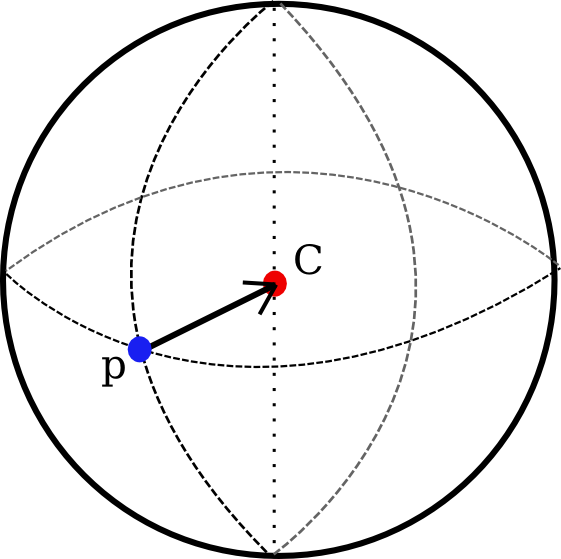
\includegraphics[scale=0.9]{informe/imagenes/esfera/esferaModelo.png} \\
    \captionof{figure}{Vemos que el vector que nos interesa es $S = c - p$}
}

$ $\newline

Mas precisamente, $S = (c_{x} - p_{x}, c_{y} - p_{y}, c_{z} - p_{z}).$ En principio no conocemos ninguno de estos valores, pero concentrémonos en calcular sobre el eje $x$ e $y$. De la imagen de la esfera (2D) podemos conocer algunos datos. En la implementación utilizamos la máscara provista por la cátedra para simplificar los cálculos. \\

Como los píxeles en la máscara son blancos o negros, es muy sencillo identificar los puntos que pertenecen a la esfera con sólo ver su color. Recorriendo todos los puntos y tomando máximos y mínimos obtenemos 4 puntos clave: El punto del círculo que está mas a arriba $A$, el más abajo $A'$, el de más a la izquierda $B$ y el de más a la derecha $B'$. \\

{\centering
    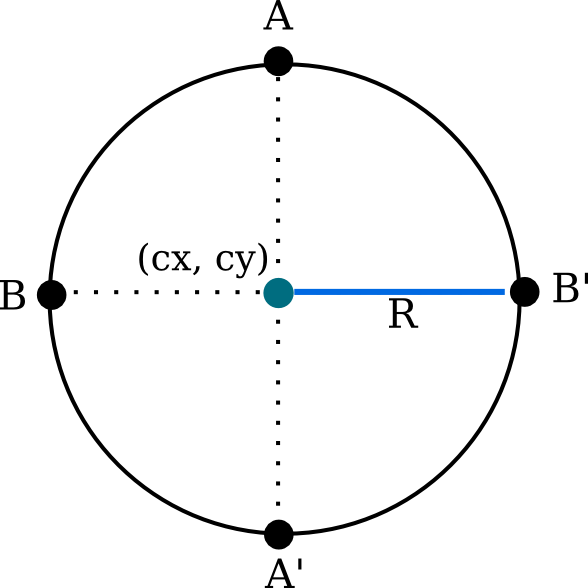
\includegraphics[scale=0.5]{informe/imagenes/esfera/circulo.png} \\
}

Puede verse fácilmente que el radio $R$ del círculo es la mitad de la distancia entre $B$ y $B'$

\begin{center}
$R = \frac{|B'_x - B_x|}{2}$.
\end{center}

Además, sabiendo que $c$ es el centro del círculo,

\begin{center}
    $c_{x} = B_x + R$ \\
    $c_{y} = A_y + R$
\end{center}

Es fácil obtener $p$ en una imagen 2D, basta con recorrer los pixeles de la imagen y quedarnos con el $(p_x, p_y)$ con mayor iluminación. Tenemos entonces los datos de $c_x$, $c_y$, $p_x$, $p_y$ y $R$. Veamos cómo podemos despejar lo que nos falta. \\

Recordemos lo que queríamos calcular:
\begin{center}
    $S = (c_{x} - p_{x}, c_{y} - p_{y}, c_{z} - p_{z}).$
\end{center}

Sólo la tercer componente de $S$ es una incógnita. Sabemos que el radio del círculo es igual al radio de la esfera y el radio de la esfera es igual a la distancia euclidea entre el centro y un punto en la superficie. En particular, el radio es igual a la distancia entre $p$ y $c$. Es decir:

\begin{center}
    $\norm{c - p} = R$ \\
\end{center}

Despejando..

\begin{center}
    $\sqrt{(c_{x} - p_{x})^{2} + (c_{y} - p_{y})^{2} + (c_{z} - p_{z})^{2}} = R$ \\ $ $

    $(c_{x} - p_{x})^{2} + (c_{y} - p_{y})^{2} + (c_{z} - p_{z})^{2} = R^{2}$ \\ $ $

    $(c_{z} - p_{z})^{2} = R^{2} - (c_{x} - p_{x})^{2} - (c_{y} - p_{y})^{2}$ \\ $ $

    $(c_{z} - p_{z}) = \sqrt{R^{2} - (c_{x} - p_{x})^{2} - (c_{y} - p_{y})^{2}}$ \\ $ $

\end{center}

Finalmente conseguimos lo que buscábamos. Repitiendo este procedimiento, podemos obtener todas las componentes del vector de luz para todas las imagenes. Podemos escribir a cualquier vector de luz utilizando datos conocidos:

\begin{center}
    $s_x = c_{x} - p_{x}$ \\
    $s_y = c_{y} - p_{y}$ \\
    $s_z = \sqrt{R^{2} - (c_{x} - p_{x})^{2} - (c_{y} - p_{y})^{2}})$ \\
\end{center}

Ya estamos en condiciones de resolver el sistema original pues conocemos todos sus coeficientes. Analizaremos en las siguientes secciones diferentes formas para resolverlo.

